\documentclass{beamer}
\usepackage[latin1]{inputenc}
\usepackage{graphicx}
\usetheme{Hannover}


\title{Implementing a Go Class Based on Gnugo}
\author{Yuzhe Zhou}

\begin{document}

\begin{frame}
\titlepage

\end{frame}

\begin{frame}
What is Go? Go is a game played on a 19*19 grid board, consists of the players alternating placing black and white stones down on the intersections of the board; If two stones of the same color are adjacent, they are "connected". If any connected group is not adjacent to any open intersections, they are captured off the board.
At the end of the game (when both players pass), you add up the total
number of open intersections your stones surround and the number of
stones from your opponent that you've captured.

\end{frame}

\begin{frame}
A typical game board in progress
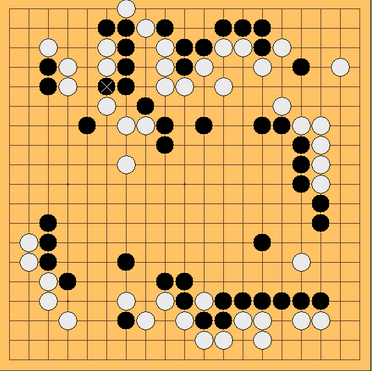
\includegraphics[scale = 0.45]{Go.png}
\end{frame}

\begin{frame}
What is Gnugo?
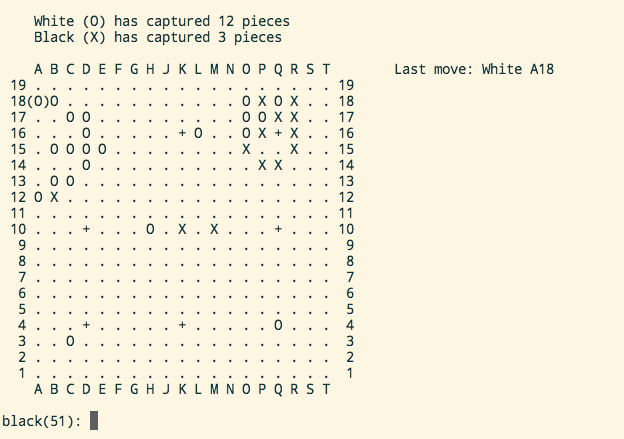
\includegraphics[scale = 0.45]{Gnugo.png}
If you type in Gnugo at the command line terminal, you can use it right now.

\end{frame}

\begin{frame}
My project aims at getting the output of a gnugo and turns it into a sage class. It now has 3 basic methods:
printboard, plot board and findstone, which gives information about the board. 
\end{frame}

\end{document}
